\chapter{Améliorations du développement logiciel}
    \section{Des outils de détection classique : quel point de départ ?}
        Comme vu en \ref{part2}, l'état de l'art en détection de vulnérabilités logicielles
        intègre déjà l'utilisation de LLM en aval de la phase de développement. Cette section
        propose une courte rétrospective des méthodes de détection de vulnérabilités classiques
        afin de mieux cerner la plus-value apportée par la détection en temps réel.
                \begin{figure}[H]
                    \centering
                    {\fbox{
                        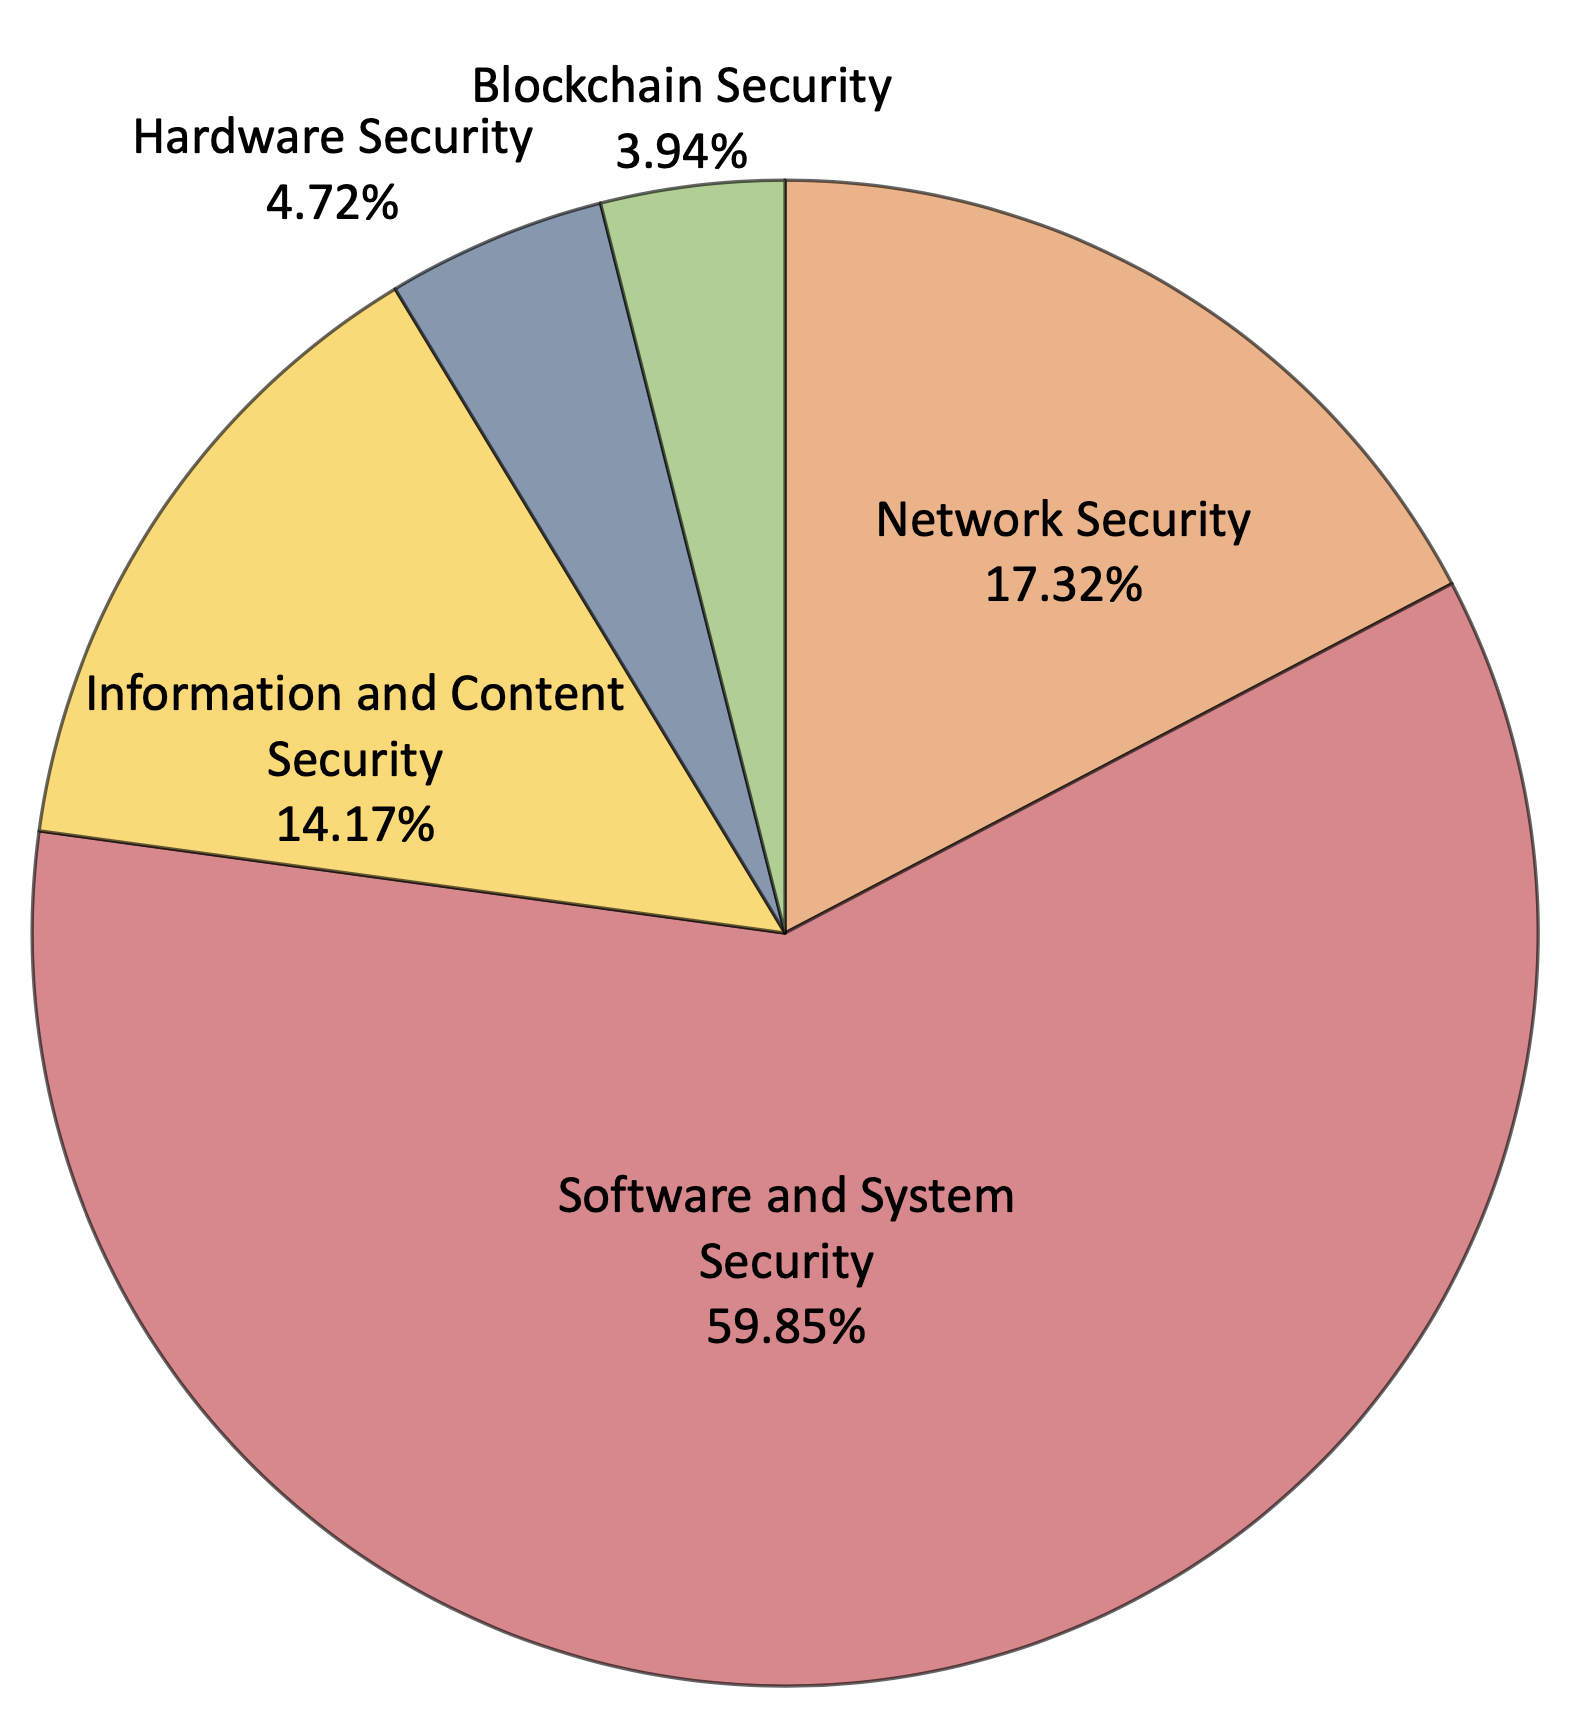
\includegraphics[width = 0.8\textwidth]{figures/Distribution of LLM usages in security domains}}}
                    \caption{Répartition de l'utilisation de LLM pour des tâches de sécurité\cite{citing4}}
                \end{figure}
        \newpage\subsection{Détection de vulnérabilités par IA : quelques outils à l'état de l'art}
            \subsubsection{Copilot}
                \texttt{Copilot} peut facilement être considéré comme le leader du développement
                assisté par LLM. Ses fonctionnalités sont nombreuses, bien éprouvées, et portées
                sur plusieurs modèles de pointe \textit{(GPT-4o, Claude 3.7 Sonnet ...)}.
                \texttt{Copilot} est désormais intégré sur de nombreux environnements de
                développement \textit{(VSCode, Suite Jetbrains ...)} et utilisé de façon quasi universelle.

                Par ailleurs, \texttt{Copilot} a servi de base de développement à un outil sorti
                en 2024 visant spécifiquement à introduire l'IA dans la cybersécurité : \texttt{Microsoft Copilot
                for Security }\footnote{https://www.youtube.com/watch?v=T3OKmtIPyzQ}. Si l'entreprise vante les
                mérites d'une analyse  évolutive en
                temps réel de l'outil\footnote{https://www.lemagit.fr/actualites/366621612/Microsoft-pousse-Security-Copilot-dans-lere-agentique}, la présente étude n'a pas trouvé de source
                mentionnant une capacité de celui-ci à détecter des vulnérabilités logicielles sur cette même
                temporalité. Cette feature est donc vraisemblablement absente ou méconnue des
                utilisateurs.
                \begin{figure}[H]
                    \centering
                    {\fbox{
                        \includegraphics[width = 0.8\textwidth]{figures/security-copilot-diagram}}}
                    \caption{Schéma conceptuel du fonctionnement de \texttt{Microsoft Copilot for Security}}
                \end{figure}
            \subsubsection{
\texttt{Snyk}, \textit{ powered by }
\texttt{Deepcode} : un exemple de standard industriel pour la sécurisation de code par IA}
                Cet outil permet de mener des analyses statiques de code à des fins spécifiques
                de sécurisation. Cependant, du propre aveu du développeur
                \footnote{https://docs.snyk.io/scan-with-snyk/snyk-code/manage-code-vulnerabilities/fix-code-vulnerabilities-automatically},
                l'outil ne propose pas systématiquement de correctif par peur de remplacer une
                vulnérabilité par une autre, ou de ne pas arriver à corriger celle identifiée.

                Par ailleurs, les analyses statiques ne permettent par définition pas à\texttt{Snyk} ne permet  pas de détecter les vulnérabilités en temps réel. Il est donc impossible d'utiliser cet outil pour corriger le code pendant la phase de développement.

        \subsection{Cas particulier du code généré par des LLM}
            Dans une perspective de nouveau paradigme de développement logiciel, il est
            important de considérer que le code revu par LLM peut également être un code généré
            par de tels modèles.

            \paragraph*{Pratiques actuelles de développement par LLM : exemple d'IntelliCode}
                %45
    \section{Correction et complétion pendant la phase de développement : promesses et difficultés rencontrées}
        %50
    \section{Interprétation des métriques de classification présentées}
        %38
